\documentclass[../../Thesis.tex]{subfiles}
\usepackage[italian]{babel}

\begin{document}
\chapter{Dataset}
Il dataset \cite{rossini2022slitherauditedcontracts} utilizzato in questo progetto è un dataset disponibile pubblicamente sulla piattaforma HuggingFace una delle più importanti piattaforme per il Natural Language Processing. HF è un'infrastruttura open-source che fornisce accesso a una vasta gamma di modelli di deep learning pre-addestrati, tra cui alcuni dei più avanzati nel campo del NLP.
Questo dataset contiene 106.474 smart contracts scritti in linguaggio Solidity un linguaggio di programmazione Touring completo divenuto lo standard per la scrittura di smart contracts su Ethereum. Ogni elemento nel dataset è composto da quattro elementi:
\begin{itemize}
    \item  \textbf{Address}: l'indirizzo del contratto
    \item  \textbf{SourceCode}: il codice sorgente del contratto
    \item  \textbf{ByteCode}: il codice bytecode del contratto
    \item  \textbf{Slither}: il risultato dell'analisi statica del contratto con Slither, è un array che contiene valori che vanno da 1 a 5. 
\end{itemize}
\subsection{Vulnerabilità}
In questo lavoro sono state prese in considerazione cinque classi di vulnerabilità diverse: 
\begin{itemize}
    \item Access-Control
    \item Arithmetic
    \item Other
    \item Reentrancy
    \item Safe
    \item Unchecked-Calls
\end{itemize}

\subsubsection{Access-Control}
La vulnerabilità di access control è una vulnerabilità presente non solo in Solidity ma in numerosi altri linguaggi di programmazione. Questa vulnerabilità si verifica quando un contratto non controlla correttamente l'accesso alle sue funzioni e ai suoi dati, è quindi una vulnerabilità legata al governanre chi può interagire con le varie funzionalità all'interno del contratto. Un esempio di questo dipo di vulnerabilità è legato alla mancata restrizione dell'accesso a funzioni di inizializzazione, ad esempio:
\begin{lstlisting}[language=Solidity]
function initContract() public {
    owner = msg.sender;
}
\end{lstlisting} 
Questa funzione serve a inizializzare l'owner del contratto, ma non controlla chi può chiamarla, permettendo a chiunque di chiamarla e diventare l'owner del contratto e non ha nemmeno controlli per prevenire la reinizializzazione. Questo è un esempio molto semplice di come una vulnerabilità di access control possa portare a comportamenti inaspettati. 
Un famoso attacco che ha subito una vulnerabilità di tipo access-control è il caso di Parity Multisig Wallet, un contratto che permetteva di creare wallet multi firma. Questo contratto ha subito un attacco nel Luglio 2017 che ha portato alla perdita di una grande quantità di Ether. L'attacco è stato effettuato da un utente che ha sfruttato una vulnerabilità di access control per diventare l'owner del contratto e rubare criptovalute ad altri utenti, si stima che la perdita sia stata di circa 30 milioni di dollari.


\subsubsection{Arithmetic}
Le vulnerabilità di tipo aritmetico \cite{sc-vulnerabilities} sono vulnerabilità che vengono generate come risultato di operazioni matematiche. Una delle vulnerabilità più significative all'interno di questa classe è rappresentata dagli underflow/overflow, un problema molto comune nei linguaggi di programmazione. Incrementi di valore di una variabile oltre il valore massimo rappresentabile o decrementi al di sotto del valore minimo rappresentabile (detti \emph{wrap around}) possono generare comportamenti indesiderati e risultati errati. In tutte le versioni di Solidity precedenti alla versione 0.8.0, le operazioni aritmetiche non controllano i limiti di overflow e underflow previsti per quel tipo di dato (es.uint64 o uint256), permettendo a un attaccante di sfruttare questa vulnerabilità per ottenere un vantaggio. Ad esempio nel caso in cui si stia utilizzano un uint256 il massimo numero che si piuò memorizzare nella variabile è $2^256 - 1$, che è un numero molto alto, ma resta comunque possibile superare questo limite, facendo entrare in scena l'overflow. Quando si verifica un overflow, il valore della variabile riparte dal piuù piccolo valore rappresentabile. Questo può portare a comportamenti inaspettati e a perdite di fondi. Vediamo un esempio molto banale di contratto vulnerabile:
\begin{lstlisting}[language=Solidity]
    pragma solidity 0.7.0;

    contract ChangeBalance {
        uint8 public balance;
        function decrease() public {
            balance--;
        }
        function increase() public {
            balance++;
        }
    }
\end{lstlisting}
Questo codice rappresenta un contratto che molto semplicemente memorizza un saldo all'interno di una variabile di tipo uint8, cioè un intero a 8bit ovvero un intero che può memorizzare valori da 0 a $2^8-1$, quindi da 0 a 255. Se un utente chiamasse la funzione \texttt{increase()} in modo tale che faccia salire il valore del saldo a $256$ il calcolo risulterebbe in un overflow e il valore della variabile ritornerebbe a 0. Questo è un esempio molto semplice di come un overflow possa portare a comportamenti inaspettati. L'underflow si verificherebbe nel caso diametralmenmte opposto, in cui viene chiamata la funzione \texttt{decrease()} quando il saldo è a 0. In questo caso il valore della variabile ritornerebbe a 255.
Un esempio di attacco che sfrutta l'overflow è stato l'attacco del 23 Aprile 2018 effettuato su uno smart contract di BeautyChain (BEC) che ha causato un importantissimo crash del prezzo. La funzione che ha causato l'overflow permetteva di trasferire una certa somma di denaro presa in input a più utenti contemporaneamnete e per farlo controllava dapprima che il saldo del contratto fosse maggiore o uguale alla somma da trasferire:
\begin{lstlisting}[language=Solidity]
    function batchTransfer(address[] _receivers, uint256 _value) public whenNotPaused returns (bool) {
        uint cnt = _receivers.length;
        uint256 amount = uint256(cnt) * _value;
        require(cnt > 0 && cnt <= 20);
        require(_value > 0 && balances[msg.sender] >= amount);
    
        balances[msg.sender] = balances[msg.sender].sub(amount);
        for (uint i = 0; i < cnt; i++) {
            balances[_receivers[i]] = balances[_receivers[i]].add(_value);
            Transfer(msg.sender, _receivers[i], _value);
        }
        return true;
     }
\end{lstlisting}
% IMAGE BECPrice
\begin{figure}[H]
    \centering
    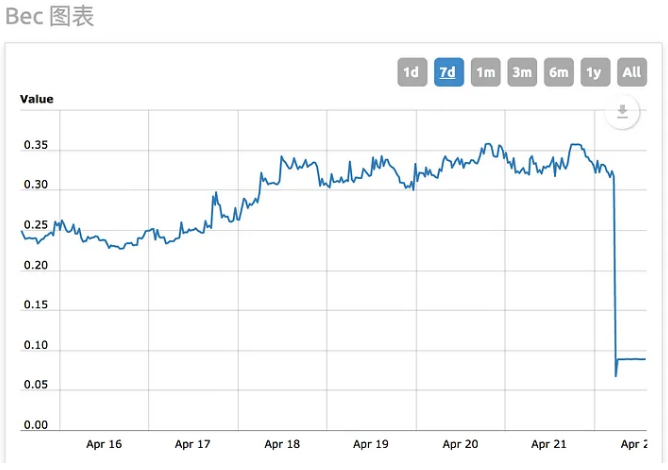
\includegraphics[width=0.8\textwidth]{../../img/BECPrice.png}
    \caption{Andamento del prezzo di BEC prima e dopo  l'attacco}
    \label{fig:BECPrice}
\end{figure}
Dalla versione di Solidity 8.0  tutti i calcoli che superano i limiti di rappresentazione del tipo di dato vengono interrotti e viene lanciata un'eccezione. Questo permette di evitare che si verifichino overflow e underflow. Un'altra soluzione a questo tipo di errori è l'utilizzo della libreria SafeMath, che offre operazioni aritmetiche che controllano i limiti di rappresentazione del tipo di dato prima di effettuare i calcoli. Overflow e underflow sono le principali vulnerabilità di tipo aritmetico, ma non sono le uniche. Un'altra vulnerabilità di tipo aritmetico è rappresentata dalla divisione per zero. In Solidity nelle versioni precedenti alla 0.4 la divisione per zero non lancia un'eccezione, ma ritorna il valore 0, questo può portare a comportamenti inaspettati e a perdite di fondi.
\subsubsection{Other}
In questa classe di vulnerabilità rientrano tutte quelle vulnerabilità che non fanno parte delle altre classi. Uno degli esempi sono le vulnerabilità di \emph{uninitialized-state} che fanno capo a tutte quelle vulnerabilità a seguito di variabili che non vengono inizializzate correttamente. Le variabili in Solidity possono essere memorizzate in \emph{memory}, \emph{storage} o \emph{calldata}. Bisogna assicurarsi che questi diversi storage vengano compresi e inizializzati correttamente, poichè ad esempio inzializzare male i puntatori allo storage o lasciarli non inizializzati può portare a degli errori. Da Solidity 0.5.0 i puntatori allo storage non inizializzati non sono più un problema poichè contratti con puntatori non inizializzati risulteranno in errori di compilazione.  
Un altra possibile vulnerabilità è detta \emph{incorrect-equality}. Questa vulnerabilità si verifica, solitamente, quando si controlla affinche un account ha abbastanza Ether o Tokens utilizzando una uguaglianza stretta, ciò è un qualcosa che un soggetto malevolo può facilmente manipolare per attaccare il contratto. Un esempio di questo tipo di vulnerabilità è il caso in cui il contratto entra in uno stato di \emph{GridLock}:
\begin{lstlisting}[language=Solidity]
    /**
    * @dev        Locks up the value sent to contract in a new Lock
    * @param      term         The length of the lock up
    * @param      edgewareAddr The bytes representation of the target edgeware key
    * @param      isValidator  Indicates if sender wishes to be a validator
    */
   function lock(Term term, bytes calldata edgewareAddr, bool isValidator)
       external
       payable
       didStart
       didNotEnd
   {
       uint256 eth = msg.value;
       address owner = msg.sender;
       uint256 unlockTime = unlockTimeForTerm(term);
       // Create ETH lock contract
       Lock lockAddr = (new Lock).value(eth)(owner, unlockTime);
       // ensure lock contract has all ETH, or fail
       assert(address(lockAddr).balance == msg.value); // BUG
       emit Locked(owner, eth, lockAddr, term, edgewareAddr, isValidator, now);
   }
\end{lstlisting}
In questo caso la vulnerabilità è rappresentata dall'assert che controlla che il contratto abbia ricevuto la quantità di Ether corretta. Il controllo si basa sull'assunzione che il contratto essendo creato alla riga precedente abbia saldo zero ed essendo precaricato proprio con \emph{msg.value} si suppone che il saldo del contratto sia uguale a \emph{msg.value}. In realtà gli Ether possono essere inviati ai contratti prima che vengano istanziati negli indirizzi stessi, poichè la generazione degli indirizzi dei contratti in Ethereum è un processo basato su dei nonce deterministici. L'attacco DoS che si basa su questa vulnerabilità in questo caso consiste nel pre-calcolare l'indirizzo del contatto \emph{Lock} e mandare dei Wei a quell'indirizzo. Questo forza la funzione \emph{lock} a fallire e a non creare il contratto, bloccando il contratto in uno stato di \emph{GridLock}.  Per risolvere questa problematica, si potrebbe adottare l'approccio di sostituire l'uguaglianza stretta con un confronto maggiore o uguale. 
\subsubsection{Reentrancy}
La Reentrancy è una classe di vulnerabilità presente negli SmartContracts che permette ad un malintenzionato di rientrare nel contratto in modo inaspettato durante l'esecuzione della funzione originale. Questa vulnerabilità può essere utilizzata per rubare fondi e rappresenta la vulnerabilità più impattante dal punto di vista di perdita di fondi a seguito di attacchi.
Il caso più famoso di questo attacco che lo ha anche reso noto è il caso di The DAO, un contratto che ha subito un attacco di reentrancy che ha portato alla perdita circa sessanta milioni di dollari in Ether, circa il 14\% di tutti gli Ether in circolazione all'epoca. Nonostante dal 2016 ad oggi siano stati fatti numerosi progressi nelle tecnologie e nelle misure di sicurezza questa vulnerabilità rimane comunque una delle minacce più pericolose per gli SmartContracts, poichè negli anni questo tipo di attacchi si è ripresentato notevole frequenza \cite{reentrancy-historical}. Un attacco di reentrancy può essere classificato in tre classi differenti:
\begin{itemize}
    \item \textbf{Mono-Function}: la funzione vulnerabile è la stesa che viene chiamata più volte dall'attaccante, prima del completamento delle sue invocazioni precedenti. Questo è il caso più semplice di attacco reentrancy e di conseguenza il più facile da individuare.
    \item \textbf{Cross-Function}: questo caso è molto simile al caso di mono-function Reentrancy, ma in questo caso la funzione che viene chiamata dall'attaccante non è la stessa che fa la chiamata esterna. Questo tipo di attacco è possibile solo quando una funzione vulnerabile condivide il suo stato con un'altra funzione, risultando in un una situazione fortemente vantaggiosa per l'attaccante. 
    \item \textbf{Cross-Contract}: questo tipo di attacco prende piede quando lo stato di un contratto è invocato in un altro contratto prima che viene correttamente aggiornato. Avviene solitamente quando più contratti condividono una variabile di stato comune e uno di loro la aggiorna in modo non sicuro. 
\end{itemize}
Mostreremo adesso alcuni esempi di contratti vulnerabili a questo tipo di attacco. 
\begin{lstlisting}[language=Solidity]
// UNSECURE
function withdraw() external {
    uint256 amount = balances[msg.sender];
    (bool success,) = msg.sender.call{value: balances[msg.sender]}("");
    require(success);
    balances[msg.sender] = 0;
}
\end{lstlisting}
In questo caso, il balance dell'utente viene aggiornato solo dopo che la chiamata esterna è stata completata. Questo permette all'attaccante di chiamare la funzione withdraw più volte prima che il balance venga settato a zero, permettendo all'attaccante di rubare fondi allo smart contract.
Una versione più complessa dello stesso processo è il caso cross function, di cui mostriamo un esempio:
\begin{lstlisting}[language=Solidity]
    // UNSECURE
function transfer(address to, uint amount) external {
  if (balances[msg.sender] >= amount) {
    balances[to] += amount;
    balances[msg.sender] -= amount;
  }
}

function withdraw() external {
  uint256 amount = balances[msg.sender];
  (bool success,) = msg.sender.call{value: balances[msg.sender]}("");
  require(success);
  balances[msg.sender] = 0;
}
\end{lstlisting}
In questo esempio, l'attaccante può effettuare un attacco di tipo reentrancy avendo una avendo una funzione che chiama \texttt{transfer()} per trasferire fondi spesi prima che il bilancio sia settato a zero dalla funzione \texttt{withdraw()}.
Un nuovo tipo di attacchi sono gli attacchi Read-only Reentrancy, in 
\subsubsection{Unchecked-Calls}
In solidity si possono usare delle chiamate a funzione low level come `address.call()`



\section{Exploratory Data Analysis}
Prima della costruzione dei modelli è stata affrontata una fase di analisi esplorativa dei dati. Questa fase è stata svolta per comprendere meglio la struttura del dataset e dei contratti che si andavano a classificare, per individuare eventuali problemi. 
Il dataset è diviso in tre sottoinsiemi: training, validation e test set.
Il dataset di training è composto da 79.641 contratti, il dataset di validazione da 10.861 contratti e il dataset di test da 15.972 contratti.
Per ongi entry del dataset (ogni contratto) il dataset fornisce quattro feature:
- \emph{address:} l'indirizzo del contratto 
- \emph{sourcecode:} il codice sorgente del contratto scritto in linguaggio Solidity
- \emph{bytecode:} il codice bytecode del contratto, ottenuto a partire dalla compilazione del codice sorgente utilizzando il compilatore di Solidity. Questo bytecode è quello che viene eseguito sulla macchina virtuale di Ethereum (EVM). 
- \emph{slither:} il risultato dell'analisi statica del contratto con Slither, un tool open-source per l'analisi statica di contratti scritti in Solidity. Questo risultato è un array di valori che vanno da 1 a 5, dove ogni numero  rappresenta la presenza di una vulnerabilità e 4 la sua assenza.
Tutte le informazioni sono presenti per tutti i contratti tranne l'informazione relativa al bytecode, che risulta assente per 227 contratti nel training set, 30 nel validation set e 51 nel test set. Durante la fase di preprocessing questi contratti sono stati rimossi dal dataset. 

\end{document}